% @Author: AnthonyKenny98
% @Date:   2020-04-05 18:33:38
% @Last Modified by:   AnthonyKenny98
% @Last Modified time: 2020-04-10 14:37:09
\begin{figure}[t!]
\begin{centering}
\begin{tabular}{ccc}

    \begin{subfigure}{0.3\linewidth}
    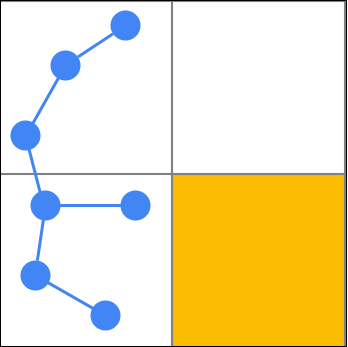
\includegraphics[width=\linewidth]{chapters/chapter2/img/keyfunctions/functions1.png}
    \caption{\texttt{getRandomConfig()}}
    \label{rrt_functions_a}
    \end{subfigure} & 

    \begin{subfigure}{0.3\linewidth}
    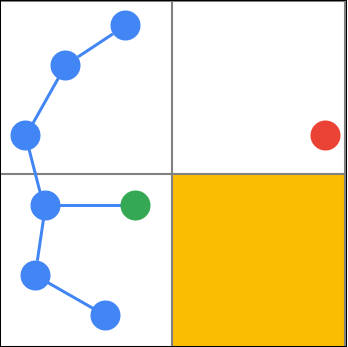
\includegraphics[width=\linewidth]{chapters/chapter2/img/keyfunctions/functions2.png}
    \caption{\texttt{findNearestConfig()}}
    \label{rrt_functions_b}
    \end{subfigure} &

    \begin{subfigure}{0.3\linewidth}
    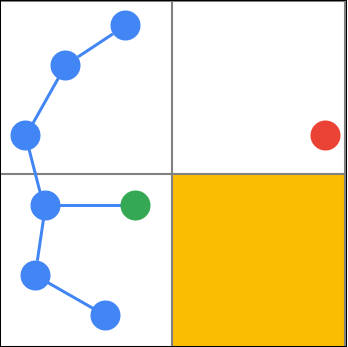
\includegraphics[width=\linewidth]{chapters/chapter2/img/keyfunctions/functions3.png}
    \caption{\texttt{stepFromNearest()}}
    \label{rrt_functions_c}
    \end{subfigure} \\

    \begin{subfigure}{0.3\linewidth}
    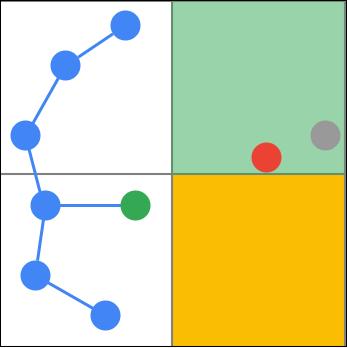
\includegraphics[width=\linewidth]{chapters/chapter2/img/keyfunctions/functions4.png}
    \caption{\texttt{configCollision()}}
    \label{rrt_functions_d}
    \end{subfigure} &

    \begin{subfigure}{0.3\linewidth}
    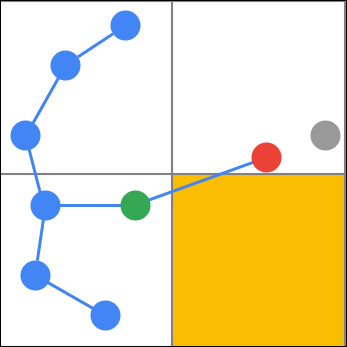
\includegraphics[width=\linewidth]{chapters/chapter2/img/keyfunctions/functions5.png}
    \caption{\texttt{edgeCollision()}}
    \label{rrt_functions_e}
    \end{subfigure} & 

    \begin{subfigure}{0.3\linewidth}
    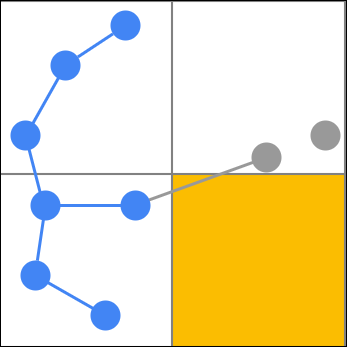
\includegraphics[width=\linewidth]{chapters/chapter2/img/keyfunctions/functions6.png}
    \caption{Discard}
    \label{rrt_functions_f}
    \end{subfigure} \\

\end{tabular}
\caption[Demonstration of the 5 Key Functions that Constitute RRT]{\textbf{Demonstration of the 5 Key Functions that Constitute RRT}, where configuration is a node in a 2D workspace. A new node is generated in (a) with \texttt{getRandomConfig()}, and the closest existing node is found with \texttt{findNearestConfig()} in (b). In this case, the new node is further than $\epsilon$ from the nearest node, and so a new node is generated with \texttt{stepFromNearest()} in (c). \texttt{configCollision()} determines that the new node is not in an occupied grid (d) and draws an edge between the two nodes. \texttt{edgeCollision()} determines that, in this case, there is a collision (e) and the new node is discarded (f).}
\label{fig:rrt_functions}
\end{centering}
\end{figure}